\documentclass[fleqn]{beamer}

\usepackage[british]{babel}
\usepackage{verbatim}
\usepackage{graphicx,hyperref,ru,url}

\title[Plaintext Recovery Attacks against SSH]{
Review: Plaintext Recovery Attacks against SSH}

\subtitle{Introduction to Cryptographic Algorithms '12/'13}

\author[Estourgie \& Br\"ucker]{
Raoul Estourgie\\
Ben Br\"ucker}

\institute[Radboud University Nijmegen]{
  Institute for Computing and Information Sciences \\
  Radboud University Nijmegen}

\date[Presentation 5-4-2013]

\begin{document}

  \begin{frame}
    \titlepage
  \end{frame}

  \begin{frame}
    \frametitle{Outline}
    \tableofcontents
  \end{frame}
  
\section{Introduction}

\subsection{What is SSH?}

  \begin{frame}
  \frametitle{What is SSH?}
    \begin{itemize}
      \item Secure Shell (SSH) connects computers securely over insecure network connections.
      \item It was released in 1995 and was designed to replace rlogin, rsh, Telnet and similar insecure protocols. 
      \item The SSH protocol covers authentication, confidentiality and integrity.
      \item Our review article "Plaintext Recovery Attacks against SSH" paper focuses on the OpenSSH implementation.
    \end{itemize}
  \end{frame}
  
\subsection{What is the SSH-BPP protocol?}

  \begin{frame}
  \frametitle{What is the SSH-BPP protocol?}
    \begin{itemize}
      \item The Binary Packet Protocol (BPP) of SSH encrypts a plaintext and then protects it's integrity by appending a MAC value.
      \item Prefixed with 4 byte packet-length, 1 byte padding-length
      \item Suffixed with 4 to 255 bytes of padding
      \item The message is then encrypted with a cypher of choice, for example aes128-cbc.
      \item MAC is calculated over this message and a 32-bit packet sequence number
      \item MAC is appended to the message
    \end{itemize}
  \end{frame}
    
  \begin{frame}
    \frametitle{Schematic of a BPP block}
    \begin{center}
    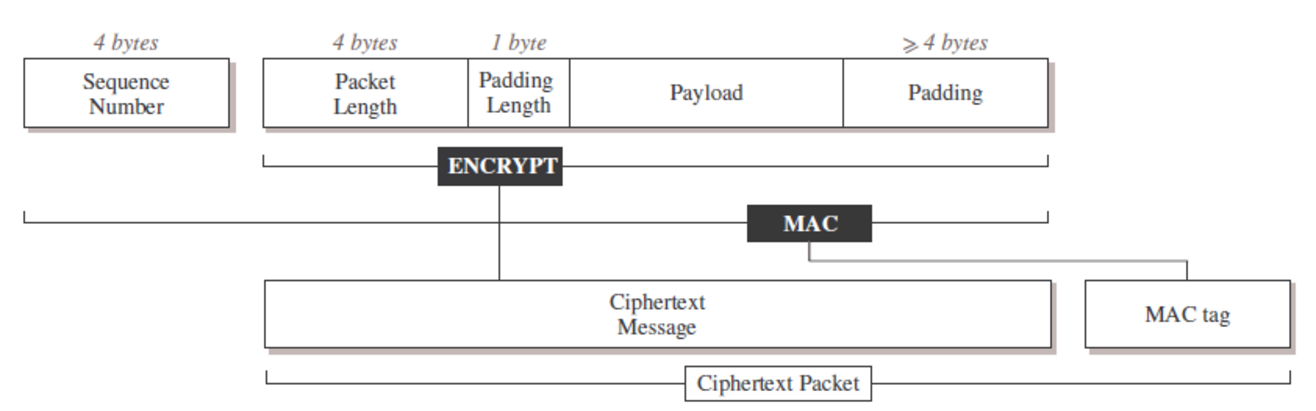
\includegraphics[scale=.4]{SSHBPP.pdf}
    \end{center}
  \end{frame}

  \begin{frame}
    \frametitle{What is the SSH-BPP protocol? cont.}
	\begin{itemize}
	\item The packets then form a data stream since the encryption is in CBC mode. 
	\item Every packet $i-1$ on a connection will be the initialization vector (IV) for packet $i$ on the same connection.
	\item For decryption it is essential that the receiver decrypts the first ciphertext block to be able to read the length field.
	\item The SSH protocol also specifies error handling for the BPP protocol. 
	\item Terminate whenever a transmission error occurs or MAC verification fails. 
	\item Implementations are free to send error messages to their peer when an error occurs.
	\end{itemize}
  \end{frame}
  
\subsection{Open SSH implementation of SSH BPP}
    \begin{frame}
  \frametitle{Open SSH implementation of SSH BPP}
\begin{center}
  
\includegraphics[scale=.2]{openssh.pdf}
\end{center}
    \begin{itemize}
      \item Open SSH first performs a length check. If the length given in the length field is not between 5 and $2^{18}$ it sends a \textit{SSH2 MSG DISCONNECTED} error back to the sender.
      \item Next OpenSSH checks that the total number of bytes expected is indeed a multiple of the block size. When this check fails, the TCP connection will terminate without an error message.
      \item When all data for the package has arrived, OpenSSH performs a MAC check. If this check fails, a \textit{Corrupted MAC on input.} error message is returned to the sender.
      \item Note that an attacker can differentiate those failure modes.
    \end{itemize}
  \end{frame}

\section{The attack}

\subsection{Some notations}

   \begin{frame}
    \frametitle{Some notations}
    \begin{block}{Key}
	    K is the key of our block cipher
    \end{block}
     \begin{block}{Encrypt/Decrypt}
	    $F_k$ and $F^{-1}_k$ are the encryption and decryption operations of the block cipher
    \end{block}
         \begin{block}{CBC Mode}
	    Given a sequence $p_1,p_2,...,p_n$ of plaintext blocks making up a packet, we have: 
$c_i = F_k(c_{i-1} \oplus p_i), i = 1,2,...,n$
where $c_0$, the Initializing Vector (IV), is the last block of the previous ciphertext. Decryption works as follows: $p_i = c_{i-1} \oplus F^{-1}_k(c_i), i = 1,2,...,n$
    \end{block}
  \end{frame}

\subsection{Stage 1: Recovering first 14 bits of plaintext}
  
   \begin{frame}
    \frametitle{Recovering first 14 bits of plaintext}
        \begin{itemize}
      \item OpenSSH implementation of BPP only supports lengths up to $2^{18}$ bits.
      \item Length field is 4 bytes long.
      \item A packet will only pass the length check if the first $32-18=14$ bits are all 0
      \item So when no \textit{SSH2 MSG DISCONNECTED} error occurs, we recovered first 14 bits of plaintext.
    \end{itemize}
   \end{frame}
 
 \subsection{Stage 2: Some more bits}
  
   \begin{frame}
    \frametitle{Recovering some more bits}
        \begin{itemize}
      \item When the ciphertext block passes the block length check we get to know more bits
      \item In case of $L = 16$ (as with AES) the we know the last 4 bits for a total of 18 bits.
      \item In case of $L = 8$ (as with 3des) the we know the last 3 bits for a total of 17 bits.
    \end{itemize}   
  \end{frame}

 \subsection{Stage 3: Recovering 32 bits of plaintext}
  
   \begin{frame}
    \frametitle{Recovering 32 bits of plaintext}
        \begin{itemize}
      \item When the first 2 check succeed, the SSH connection enters wait state.
      \item Feed random cyphertext blocks into this connection and wait after each block.
      \item When the target returns a \textit{Corrupted MAC on input.} error we know that it received enough blocks to trigger a MAC check.
      \item At this point we know exactly how long the packet length is, and therefore all 32 bits of the length-field. 
      \item Because of the chaining property of the CBC mode these 32-bits leak information about the rest of the ciphertext.
    \end{itemize}   
  \end{frame}	  

  \begin{frame}
    \frametitle{Security game}
    \begin{center}
    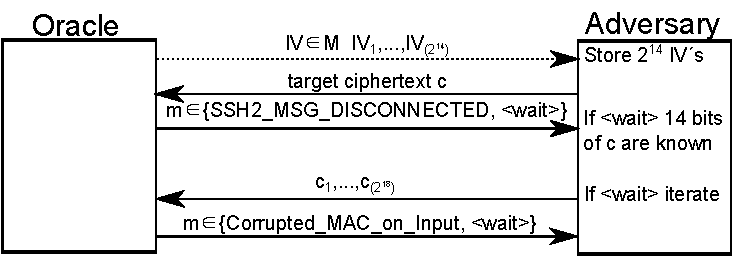
\includegraphics[scale=.8]{drawing.pdf}
    \end{center}
  \end{frame}

\section{Countermeasures}

   \begin{frame}
    \frametitle{Countermeasures}
        \begin{itemize}
      \item Return the same error message when either the length check or the block-length check failed.
      \item Randomize the length field if the length check fails.
    \end{itemize}   
  \end{frame}	

\section{Conclusion}

   \begin{frame}
    \frametitle{Conclusion}
     It is possible to recover plaintext bits from a proven secure SSH implementation. Therefore it is also hard to know whether improvements to resolve this issue won't lead to new attacks on these SSH implementations.
  \end{frame}	

\section{Questions}

  \begin{frame}
    \frametitle{Questions}
    \begin{center}
    Questions?
    \end{center}
  \end{frame}
\end{document}
